\documentclass{cheatsheet}
\usepackage{bm}
\usepackage{textcomp, mathcomp}
\usepackage{empheq}
\usepackage{pbox}
\usepackage{booktabs}
\usepackage{verbatim}
\usepackage{graphicx}
\usepackage{tabu}
\usepackage{amssymb}
\usepackage{tikz}
\usepackage{diagbox}

\doctitle{Control Systems I Cheatsheet}
\author{Christian Leser \\ \vspace*{-0.2em}}

\begin{document}
\section{1. Terminology}
	\subsection{1.1 Input, Output, State}
    %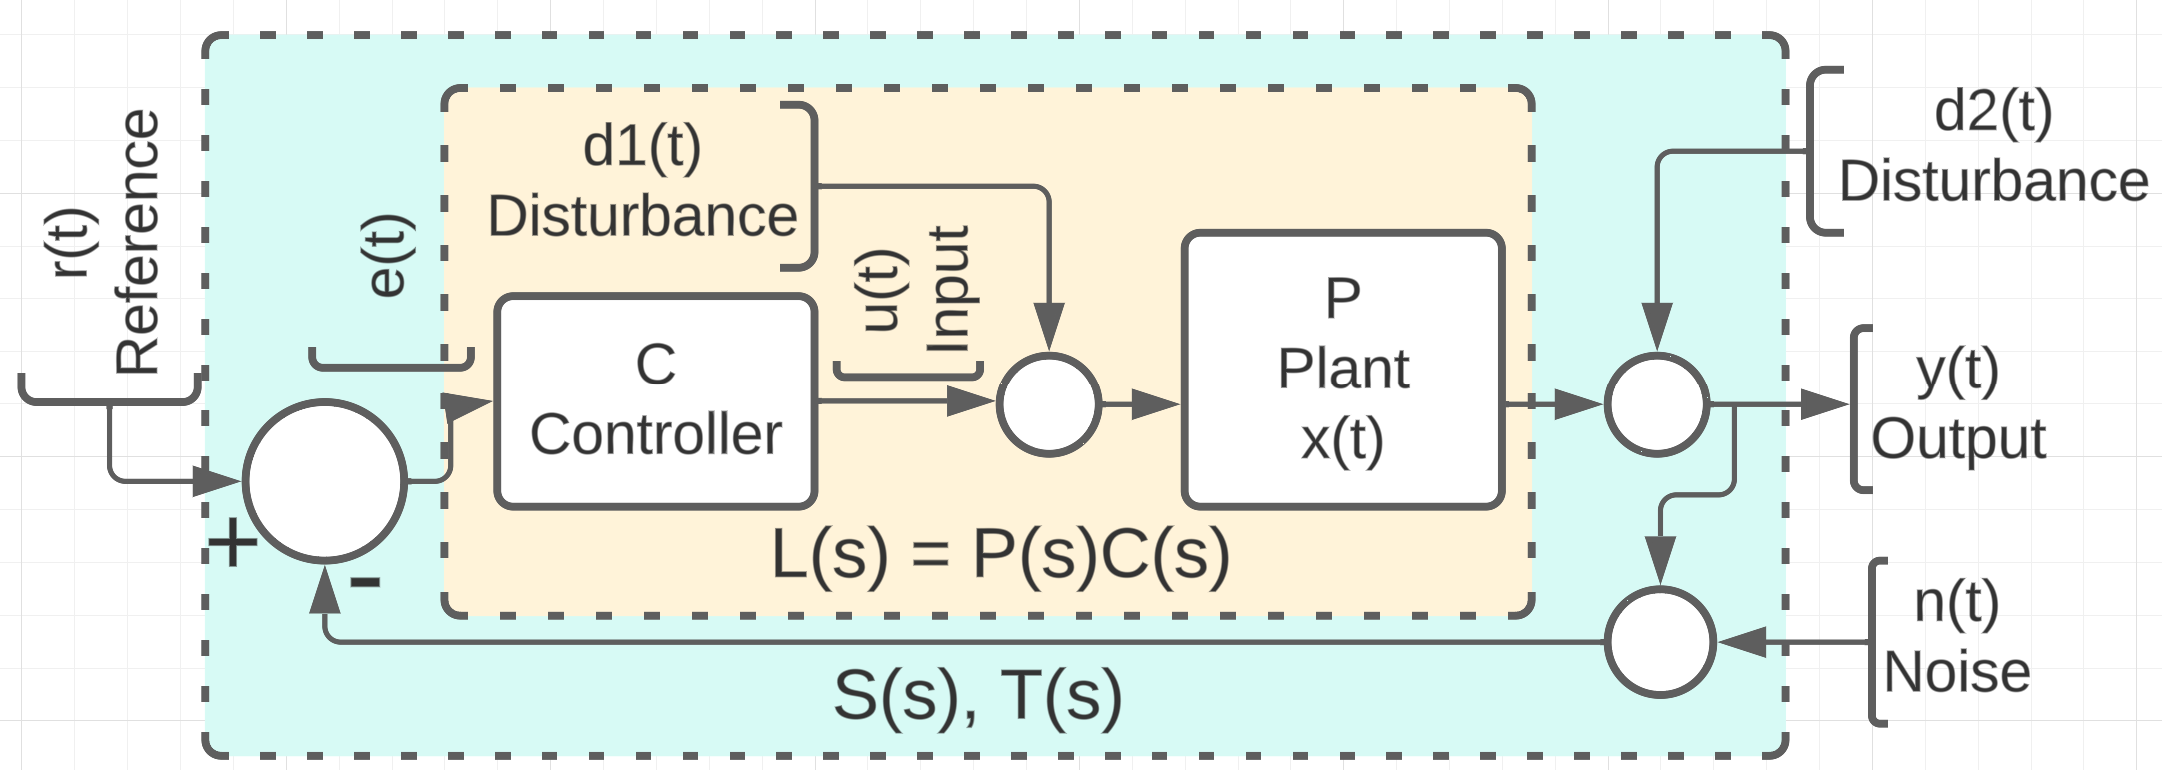
\includegraphics[width = \linewidth]{src/images/basic_block_chart.png}
    \begin{itemize}
        \item \textbf{(Control) Input u(t)} (gas pedal)
        \begin{itemize}
            \item endogenous: manipulation by designer
            \item exogenous: generated by environment (e.g. Weather)
        \end{itemize}
        \item \textbf{Output / Measurement y(t)} (speed)
        \begin{itemize}
            \item measured outputs: Quantities that we can measure
            \item performance outputs: unmeasurable but controllable (e.g. average fuel consumption)
        \end{itemize}
        \item \textbf{state x(t)}: "memory", summary of all past inputs (fuel)
        \item parameter: quantities that do not change over time (colour)
\end{itemize}
	\subsection{Classification}
    \textcolor{blue}{L}\textcolor{orange}{TI} \textcolor{teal}{SISO}: \textcolor{blue}{Linear} \textcolor{orange}{Time invariant} \textcolor{teal}{single input single output}
    \subsubsection*{Linear vs. nonlinear Systems}
        For a linear system, Additivity and Homogenity must hold:
        \begin{align*}
            \Sigma (\alpha u_a + \beta u_b) = \alpha (\Sigma u_a) + \beta (\Sigma u_b) = \alpha y_a + \beta y_b
        \end{align*}
        Therefore, superposition holds for linear systems.\\
        Linear System can be represented in state-space-form, the matrices do not depend on time:
        \begin{equation}\label{eqn:LTI}
            \begin{cases}
                \dot{x}(t) = Ax(t) + Bu(t)\\
                y(t) = Cx(t) + Du(t)
            \end{cases}
        \end{equation}

    \subsubsection*{Causal vs non-causal systems}
        Output at time $t$ depends only on the values of input on $(-\infty, t]$ (future inputs do not affect current output)\\
        $y(t) = f(u(\tau)), \tau < t$
    
    \subsubsection*{Static systems}
        Static (memoryless) vs Dynamic
        y(t) only depends on u(t), output does not depend on past or future\\
        $dim(x) = 0$ : dimension of system equals 0

    \subsubsection*{Time invariant vs Time-varying !überarbeiten!}
        output does not depend on time, only on $\Delta t$ (counter example sun clock)\\
        {\centering\textbf{\underline{Time-varying}}}
        \begin{equation}
            t_0 = t_0
            \begin{cases}
                \dot{x}(t) = f(t, x(t), u(t))\\
                y(t) = g(t, x(t), u(t))
            \end{cases}
            \rightarrow
            \begin{cases}
                \dot{x}(t) = A(t)x(t) + B(t)u(t)\\
                y(t) = C(t)x(t) + D(t)u(t)
            \end{cases}
        \end{equation}

        {\centering\textbf{\underline{Time Invariant}}}
        \begin{align*}
            \text{time shift operator $\sigma_{\tau}$:\quad \quad} \sigma_{\tau} y(t) = \Sigma \sigma_{\tau} u(t)\\
            y(t - \tau) = \Sigma(u(t - \tau))\\
            t_0 = 0
            \begin{cases}
                \dot{x}(t) = f(x(t), u(t))\\
                y(t) = g(x(t), u(t))
            \end{cases}
            \rightarrow
            \begin{cases}
                \dot{x}(t) = Ax(t) + Bu(t)\\
                y(t) = Cx(t) + Du(t)
            \end{cases}
        \end{align*}
	\subsection{Interconnections}
    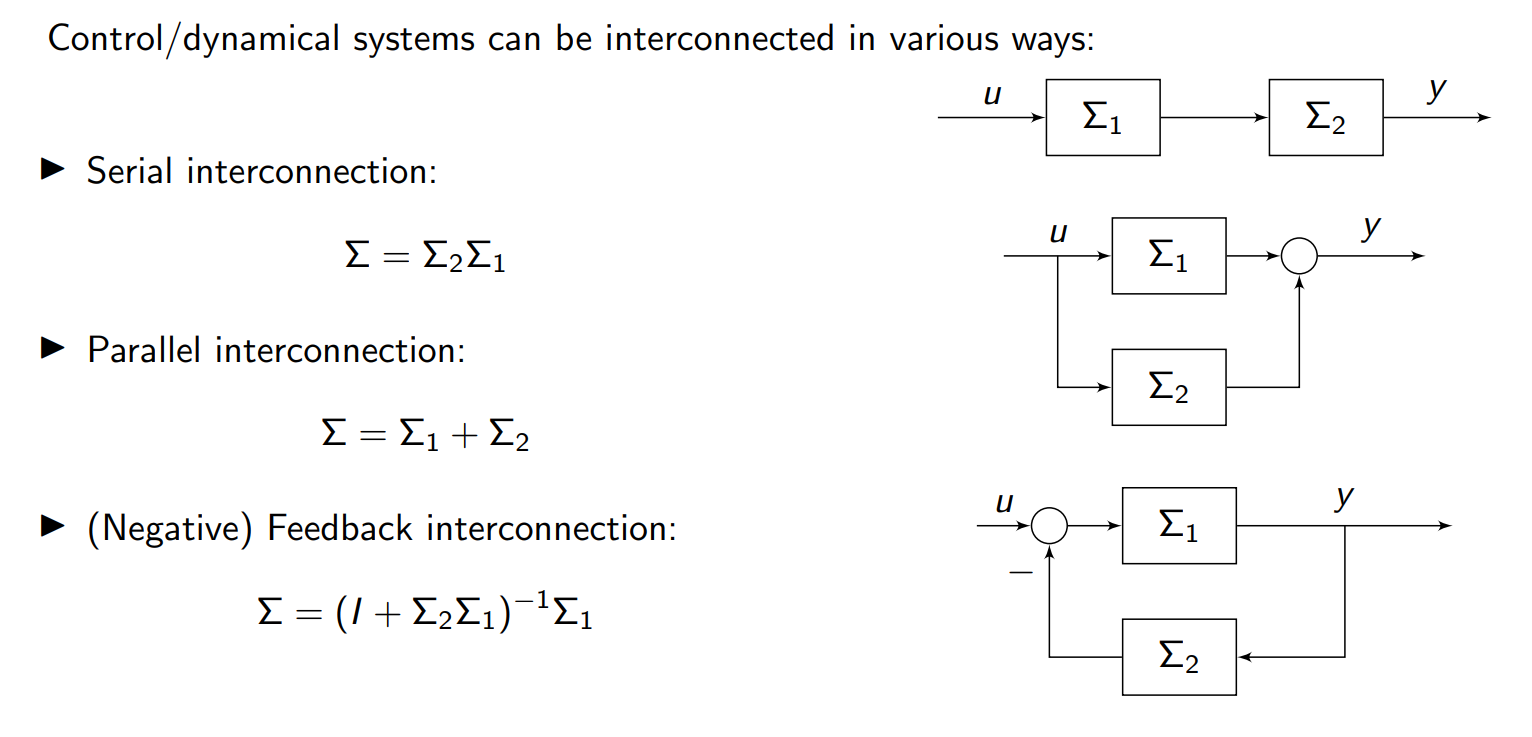
\includegraphics[width = \linewidth]{src/images/interconnection.png}
%	\subsection{Basic Control Architectures}
    \begin{tabu}{X[m] X[2, c, m]}
        \textbf{Name}               & \textbf{Block chart}\\
        \hline \hline
        Feed-forward      & 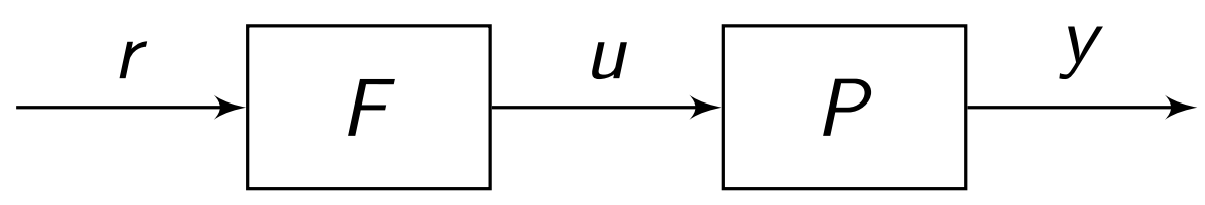
\includegraphics[width = \linewidth]{src/images/architecture_feed_forward.png}\\
        \hline
        Feedback    & 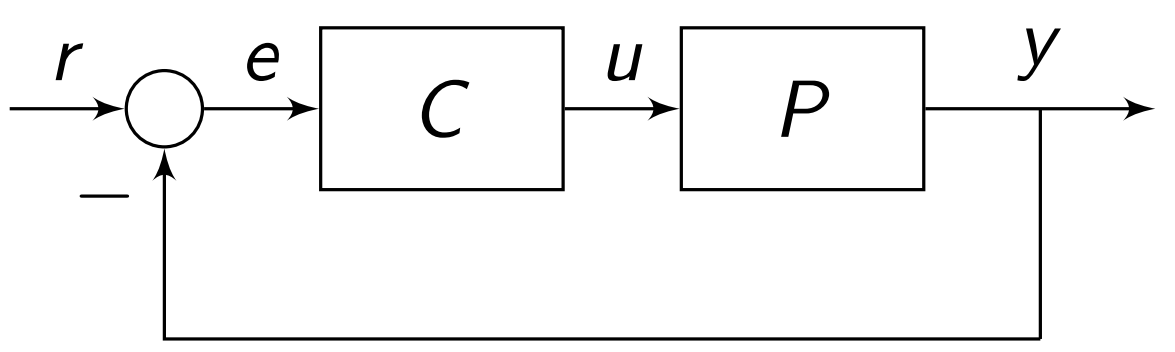
\includegraphics[width = \linewidth]{src/images/architecture_feedback.png}\\
        \hline
        Two degrees of freedom    & 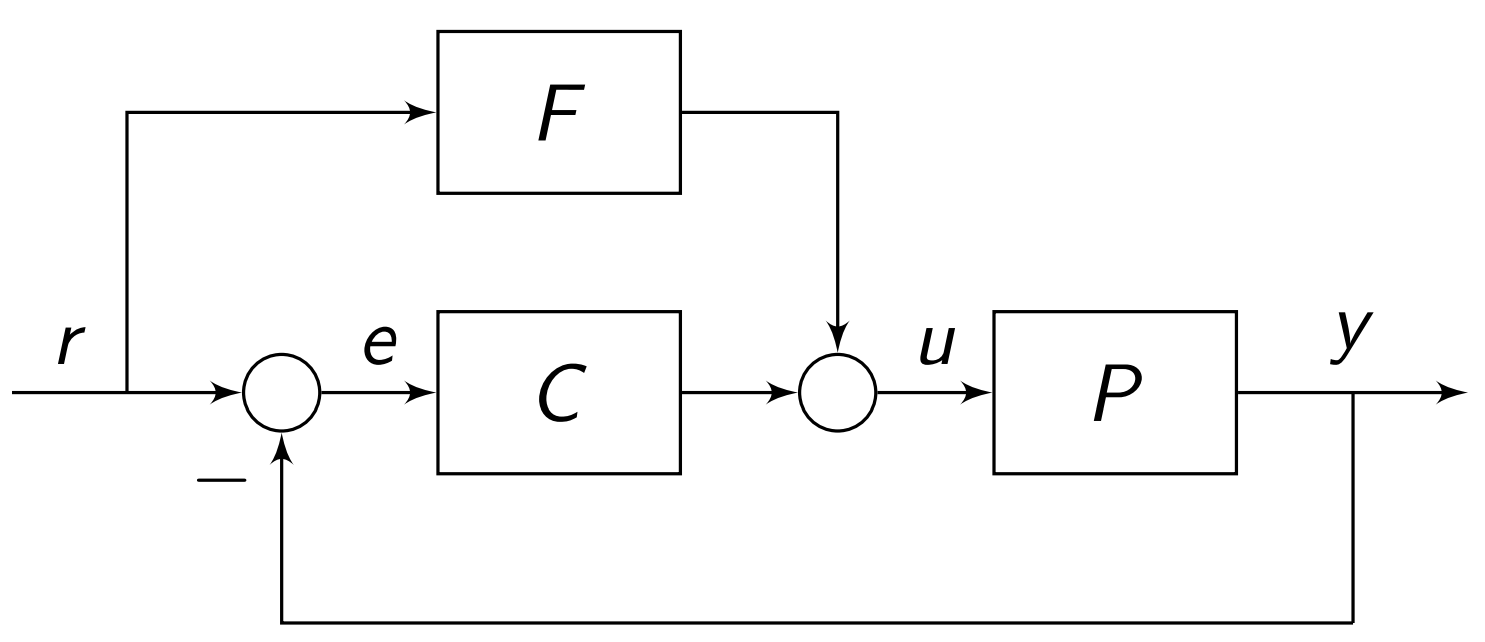
\includegraphics[width = \linewidth]{src/images/architecture_two_freedom.png}
    \end{tabu}

\section{2. System Modeling}
	for LTI SISO systems: $\frac{d}{dt} \text{storage} = \sum \text{inflows} - \sum \text{outflows}$

    \begin{center}
        \textbf{\underline{Mass conservation}}    
    \end{center}
    \begin{align*}
        \frac{d}{dt} m = \sum m_{in}(t) - \sum m_{out}(t)
    \end{align*}

    \begin{center}
        \textbf{\underline{Mechanical systems}}    
    \end{center}
    \begin{align*}
        M(t) = J \cdot \ddot{\phi}(t)
    \end{align*}

    \begin{center}
        \textbf{\underline{Thermodynamic systems}}    
    \end{center}
    \begin{align*}
        m \frac{d}{dt} T(t) = c(T_{ext}(t) -T(t)) + u(t)
    \end{align*}
	\subsection{State Space Form}
    \begin{minipage}{0.49 \linewidth}
        \begin{center}
            \textbf{\underline{General form}}
        \end{center}
        \begin{align*}
            \begin{cases}
                \dot{x}(t) = f(x(t), u(t), d(t))\\
                y(t) = f(x(t), u(t), d(t))
            \end{cases}
        \end{align*}
    \end{minipage}
    \begin{minipage}{0.49 \linewidth}
        \begin{center}
            \textbf{\underline{Linear System}}
        \end{center}
        \begin{align*}
            \begin{cases}
                \dot{x}(t) = Ax(t) + Bu(t)\\
                y(t) = Cx(t) + Du(t)
            \end{cases}\\
        \end{align*}
    \end{minipage}
    dim$(x) = $ Order/Dimension (min. $\#$ of variables to describe state)
    
	\subsection*{Jacobian Linearization Process}
    Use in LTI-Systems\\
    Equilibrium point (state does not change): $\dot{x} = f(x_e, u_e) = 0$\\
    Linearized systems are accurate around equilibrium:
    \begin{align*}
        \left(
            \begin{array}{c}
                x\\
                u
            \end{array}
        \right)
        \approx
        \left(
            \begin{array}{c}
                x_e\\
                u_e
            \end{array}
        \right)
    \end{align*}
    \begin{align*} % \Big\rvert_{x = x_e, u = u_e} Auswertung der Differentiale
        A &= 
        \left[\begin{array}{c c c}
            \frac{\partial f_1}{\partial x_1} & \cdots & \frac{\partial f_1}{\partial x_n}\\
            \vdots & \ddots & \vdots\\
            \frac{\partial f_n}{\partial x_1} & \cdots & \frac{\partial f_n}{\partial x_n}
        \end{array}\right]
        &B &= 
        \left[\begin{array}{c}
            \frac{\partial f_1}{\partial u}\\
            \vdots\\
            \frac{\partial f_n}{\partial u}
        \end{array}\right]
        \\
        C &= 
        \left[\begin{array}{c c c}
            \frac{\partial g}{\partial x_1} & \cdots & \frac{\partial g}{\partial x_n}
        \end{array}\right]
        &D &= 
        \left[\begin{array}{c}
            \frac{\partial g}{\partial u}
        \end{array}\right]
    \end{align*}
	\subsection{time response to LTI system}
    \begin{center}
        \textbf{Superposition of responses:}
    \end{center}
    
    \begin{minipage}{0.49\linewidth}
        \begin{minipage}{0.49\linewidth}
            non-zero initial conditions (natural response)
        \end{minipage}
        \begin{minipage}{0.49\linewidth}
            \begin{align*}
                \begin{cases}
                    x(0) = x_0\\
                    u(t) = 0
                \end{cases}
            \end{align*}
        \end{minipage}
    \end{minipage}
    \begin{minipage}{0.49\linewidth}
        \begin{minipage}{0.44\linewidth}
            non-zero inputs (forced response)
        \end{minipage}
        \begin{minipage}{0.54\linewidth}
            \begin{align*}
                \begin{cases}
                    x(0) = 0\\
                    u(t) = u(t)
                \end{cases}
            \end{align*}
        \end{minipage}
    \end{minipage}
    \begin{align*}
        x(t) &= \underbrace{e^{At} \cdot x_0}_{\substack{\text{hom. solution}\\ u(t) = 0}} + \underbrace{\int\limits_0^t e^{A (t-\rho)} B u(\rho) d\rho}_{\substack{\text{inhom. solution, zero initial condition}\\ x(0) = 0}}\\
        y(t) &= \underbrace{C \cdot e^{At} \cdot x_0}_{\substack{\text{natural / initial} \\ \text{condition response}}} + \underbrace{C \cdot \int\limits_0^t e^{A (t-\rho)} B u(\rho) d\rho}_{\text{forced response}} + \underbrace{D u(t)}_{\text{feedthrough}}
    \end{align*}

    state transition function: $\psi(t) = e^{At}$ %Maybe how to get the solution of an lti? see lecture 4 Time response
	\subsection{Stability}
    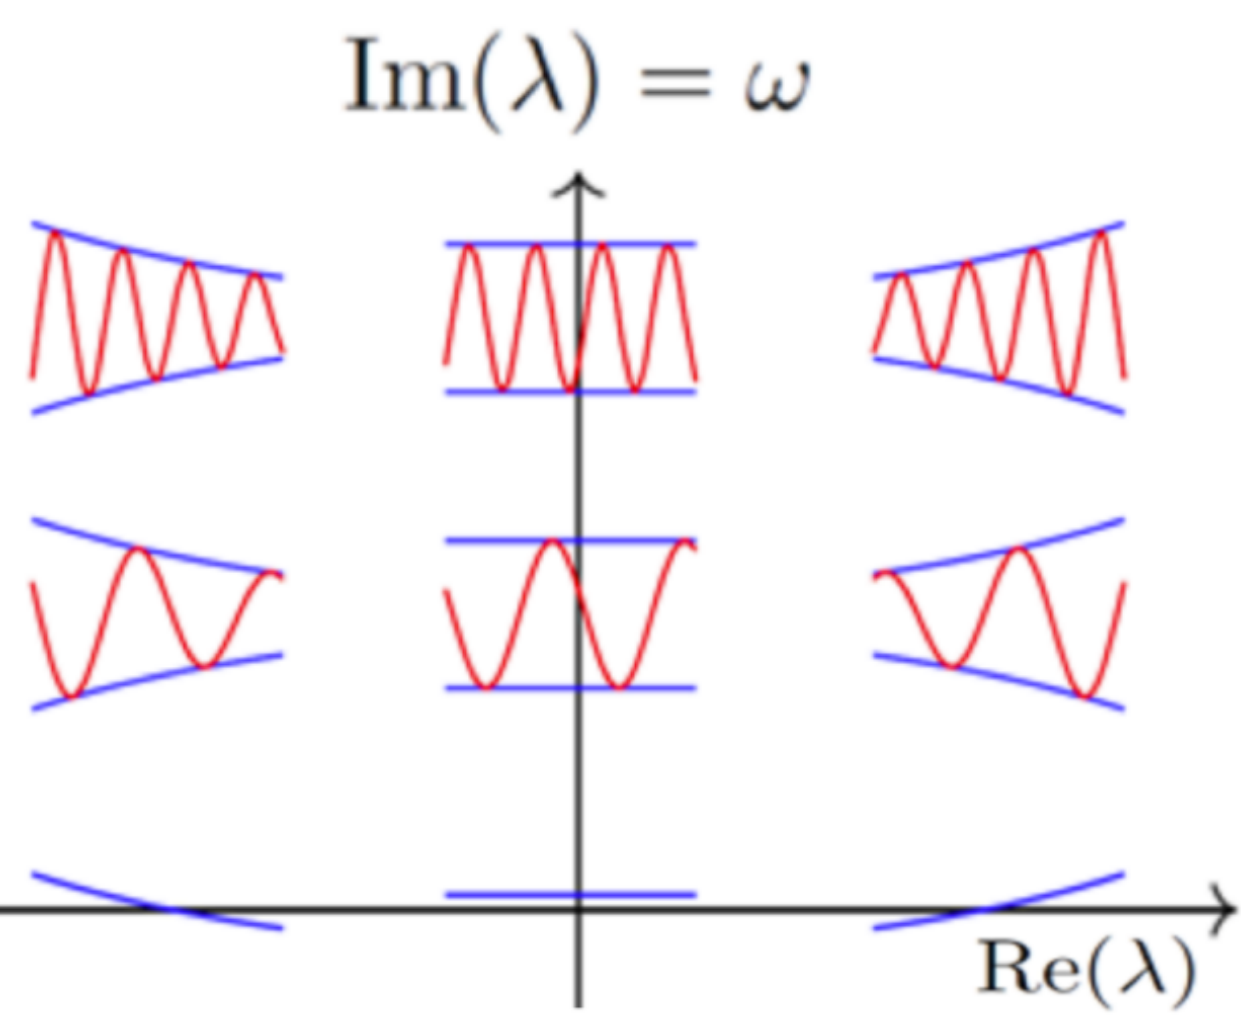
\includegraphics[width = \linewidth]{src/images/eigenvalue_response.png}
    system behaviour based on eigenvalues of A

    \subsubsection{Lyapunov stable}
    $\lim_{t \rightarrow \infty} x(t) \neq \pm \infty \Leftrightarrow Re(\lambda_i) \leq 0 \text{, exactly one } Re(\lambda_i) = 0$

    \subsubsection{Asymptotically stable}
    $\lim_{t \rightarrow \infty} x(t) = 0 \Leftrightarrow Re(\lambda_i) < 0$

    \subsubsection{BIBO (Bounded Input Bounded Output) stability}
    $\lim_{t \rightarrow \infty} y(t) \neq \pm \infty \Leftrightarrow Re(\lambda_i) < 0$

    \begin{center}
        \textbf{Not stabilizable and observable systems}
    \end{center}
    \begin{tabu}{|X[6] X X[3]|}
        \hline
        asymptotically stable & $\rightarrow$ & BIBO stable\\
        ? & $\leftarrow$ & BIBO stable\\
        Lyap. stable or unstable & $\rightarrow$ & ?\\
        Lyap. stable or unstable & $\leftarrow$ & BIBO unstable\\
        \hline
    \end{tabu}

    \subsubsection{Unstable}
    $\lim_{t \rightarrow \infty} x(t) = \pm \infty \Leftrightarrow Re(\lambda_i) > 0 \text{for at least one i}$
	\subsection{Frequency response / domain (time $\rightarrow$ frequency)}
choose $u(t) = e^{st}$ where s is a complex number\\
$ y(t) = \underbrace{Ce^{At} [x(0) - (sI - A)^{-1} B]}_{\text{Transient response (= 0 if as. stable)}}
+ \underbrace{[C(sI - A)^{-1} B + D]e^{st}}_{\text{steady-state response}}$\\
\begin{minipage}{0.39\linewidth}
    \begin{align*}
        \Rightarrow y_{ss} = G(s) e^{st}\\
    G(s) = \frac{Y(s)}{U(s)}\\
    = C(sI - A)^{-1} B + D\\
    = \frac{C \cdot \text{Adj}(sI - A) \cdot B}{\text{det}(sI - A)} + D
    \end{align*}
\end{minipage}
\begin{minipage}{0.59\linewidth}
    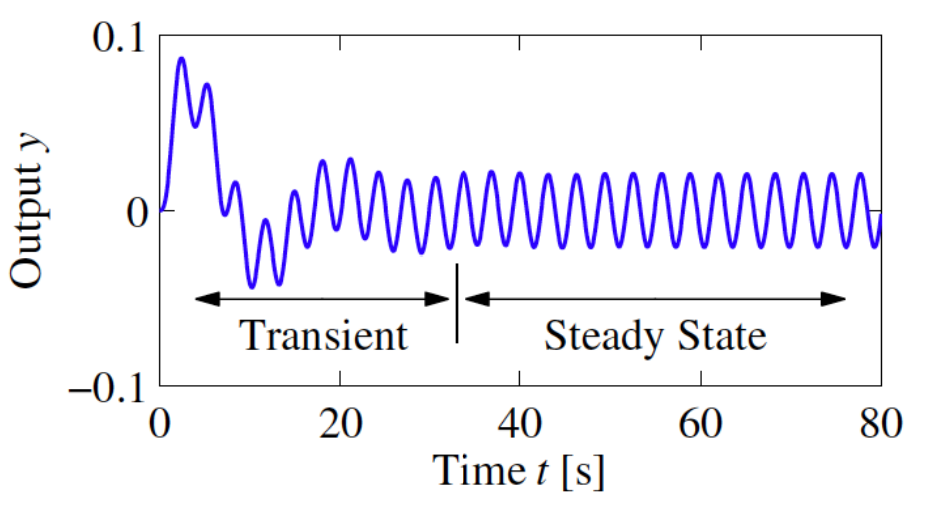
\includegraphics[width = \linewidth]{src/images/transient_steady_state.png}
\end{minipage}


\begin{align*}
    \text{adj}\left[
        \begin{array}{c c}
            a & b\\
            c & d            
        \end{array}
    \right]
    = \left[
        \begin{array}{c c}
            d & -b\\
            -c & a
        \end{array}
    \right]
    \\
    \text{adj}\left[
        \begin{array}{c c c}
            a & b & c\\
            d & e & f\\
            g & h & i
        \end{array}
    \right]
    = \left[
        \begin{array}{c c c}
            ei-fh & ch-bi & bf-ce\\
            fg-di & ai-cg & cd-af\\
            dh-eg & bg-ah & ae-bd            
        \end{array}
    \right]
\end{align*}
	\subsection{Writing the transfer function G(s)}
    \titel{Partial fraction expansion}
        \begin{align*}
            G(s) = \frac{r_1}{s-p_1} + \frac{r_2}{s-p_2} + \ldots + \frac{r_n}{s-p_n} + r_0
        \end{align*}
        $p_1, \ldots, p_n =$ poles, $r_1, \ldots, r_n =$ residues
    \titel{Root-locus}
        \begin{align*}
            G(s) &= \frac{k_{\text{rl}}}{s^q} \frac{(s-z_1)(s-z_2) \dots (s-z_m)}{(s-p_1)(s-p_2) \dots (s-p_{n-q})}
        \end{align*}
    \titel{Bode form}
        \begin{align*}
            G(s) &= \frac{k_{\text{bode}} \cdot k_{\text{rl}}}{s^q} \frac{(\frac{s}{-z_1} + 1)(\frac{s}{-z_2} + 1) \dots (\frac{s}{-z_m} + 1)}{(\frac{s}{-p_1} + 1)(\frac{s}{-p_2} + 1) \dots (\frac{s}{-p_{n-q}} + 1)}\\
            k_{\text{bode}} &= \frac{(-z_1)(-z_2) \dots (-z_m)}{(-p_1)(-p_2) \dots (-p_{n-q})}, k_{\text{bode}} \cdot k_{\text{rl}} = \underbrace{y_{ss}(t) = G(0)}_{\text{for stable systems}}
        \end{align*} 
	\subsection{Compute phase and magnitude of transfer function}
\begin{align*}
    u(t) &= sin(\omega t) \rightarrow y_{ss}(t) = \left|G(j \omega)\right| \sin\left(\omega t + \angle(G(j \omega))\right)\\
    G(s) &= k \frac{(s-z_1)(s-z_2)}{(s-p_1)(s-p_2)} \Rightarrow
    |G(s)| = k \frac{|s-z_1| \cdot |s-z_2|}{|s-p_1| \cdot |s-p_2|}\\
    \angle(G(s)) &= \angle(s-z_1) + \angle(s-z_2) - \angle(s-p_1) - \angle(s-p_2)
\end{align*}
	% 9_calculate_poles_and_zeros.tex
	% 10 Visualization in complex plane
	\subsection{controllable canonical form (frequency $\rightarrow$ time)}
\titel{$A$ is diagonal:}
\begin{align*}
    G(s) = \frac{p_1}{s-\lambda_1} + \frac{p_2}{s-\lambda_2} + ... + \frac{p_n}{s-\lambda_n} + d\\
    A = \left[\begin{array}{c c c}
        \lambda_1 & & \\
         & \ddots & \\
         & & \lambda_n
    \end{array}\right]
    ,
    B = \left[\begin{array}{c}
        \sqrt{p_1}\\
        \vdots\\
        \sqrt{p_n}
    \end{array}\right]
    \\
    C = \left[\begin{array}{c c c}
        \sqrt{p_1} & \cdots & \sqrt{p_n}
    \end{array}\right]
    ,
    D = d
\end{align*}

\titel{general case:}
\begin{align*}
    G(s) &= \frac{b_{n-1}s^{n-1} + b_{n-2}s^{n-2} + \dots + b_0}{s^n + a_{n-1}s^{n-1} + \dots + a_0} + d\\
    A &= \left[\begin{array}{c c c c c}
        0 & 1 & 0 & \cdots & 0\\
        0 & 0 & 1 & \cdots & 0\\
        \vdots & \vdots & & \ddots & 1\\
        -a_0 & -a_1 & \cdots & & -a_{n-1}
    \end{array}\right]
    ,
    B = \left[\begin{array}{c}
        0\\
        0\\
        \vdots\\
        1
    \end{array}\right]
    \\
    C &= \left[\begin{array}{c c c c}
        b_0 & b_1 & \cdots & b_{n-1}
    \end{array}\right]
    ,
    D = d
\end{align*}
	\subsection{poles and zeroes}
\begin{itemize}
    \item complex poles: oscillating system $(\omega \propto Im(p))$
    \item complex poles and zeros: always complex conjugate pairs
    \item stable pole: $Re(p) < 0$
    \item minimum-phase zero: $Re(z) < 0 \rightarrow$ overshoot
    \item minimum-phase zero, $Re(z) = 0$: zero slope at $t_0$
    \item non-minimum-phase zero: $Re(z) > 0 \rightarrow$ undershoot
\end{itemize}
	%differentiator and integrator (Lecture 5 Page 24, 25, Lecture 6 page 31, 32)
	
\section{System Analysis}
	\subsection{System response}
    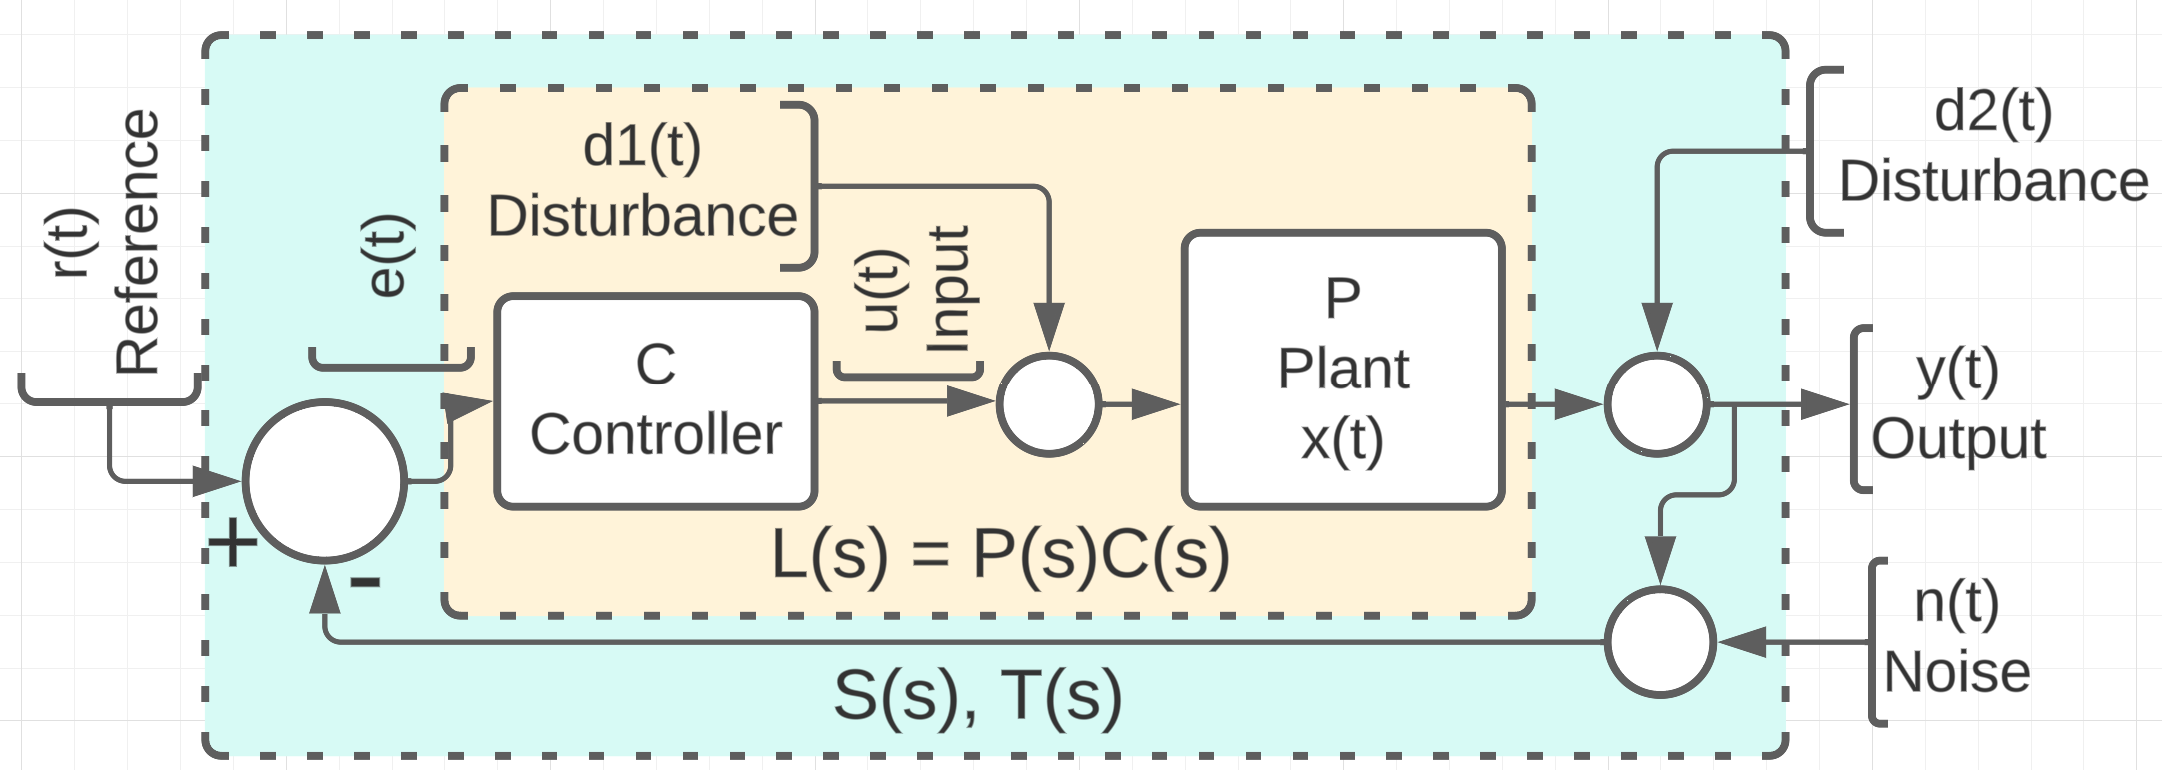
\includegraphics[width = \linewidth]{src/images/basic_block_chart.png}
    \begin{minipage}{0.49\linewidth}
        \titel{Sensitivity}
        \begin{center}
            $S(s) = \frac{1}{1 + L(s)}$
        \end{center}
    \end{minipage}
    \begin{minipage}{0.49\linewidth}
        \titel{Complimentary Sensitivity}
        \begin{center}
            $S(s) = \frac{L(s)}{1 + L(s)}$
        \end{center}
    \end{minipage}
    
    \subsubsection{steady state error, disturbance and noise}
    find steady state using final value theorem $\lim\limits_{t \rightarrow \infty} a(t) = \lim\limits_{s \rightarrow 0} A(s)$
    \begin{minipage}{0.32\linewidth}
        \begin{align*}
            e(t) = S(s) r(t)\\
            e(t) = - S(s) d_2(t)
        \end{align*}
    \end{minipage}
    \begin{minipage}{0.32\linewidth}
        \begin{align*}
            e(t) = - S(s) n(t)\\
            e(t) = - T(s) d_1(t)
        \end{align*}
    \end{minipage}
    \begin{minipage}{0.32\linewidth}
        \begin{align*}
            y(t) = T(s) r(t)
        \end{align*}
    \end{minipage}

    \subsubsection{Steady State error to Ramp reference Inputs}
        Ramp is obtained by integrating step q-times:
        \begin{align*}
            r(t) = \frac{1}{s^q}\\
            \rightarrow e_{ss} = \lim\limits_{s \rightarrow 0} \left( \frac{1}{1 + L(s)} \cdot \frac{1}{s^q} \right)\\
            L(0) = \frac{k_{\text{Bode}}}{s^q}
        \end{align*}
        knowing Type (number of poles at origin of $L(s)$) and order $q$ of ramp:\\
        \begin{tabu}[width = \linewidth]{| X | X | X | X |}
            \hline
            $e_{ss}$    & $q = 0$                           & $q = 1$                       & $q = 2$\\
            \hline \hline
            Type 0      & $\frac{1}{1 + k_{\text{Bode}}}$   & $\infty$                      & $\infty$\\
            \hline
            Type 1      & $0$                               & $\frac{1}{k_{\text{Bode}}}$   & $\infty$\\
            \hline
            Type 2      & $0$                               & $0$                           & $\frac{1}{k_{\text{Bode}}}$
        \end{tabu}
	\subsection{Step responses}
    \subsubsection{First Order System}
        \begin{align*}
            G(s) = \frac{1}{\tau s + 1} \Leftrightarrow 
            \begin{cases*}
                \dot{x} = -\frac{1}{\tau} x + \frac{1}{\tau} u\\
                y = x
            \end{cases*}\\
            \Rightarrow y(t) = 1-e^{-t/\tau}\\
            T_d = \tau \ln(100/d)
        \end{align*}
        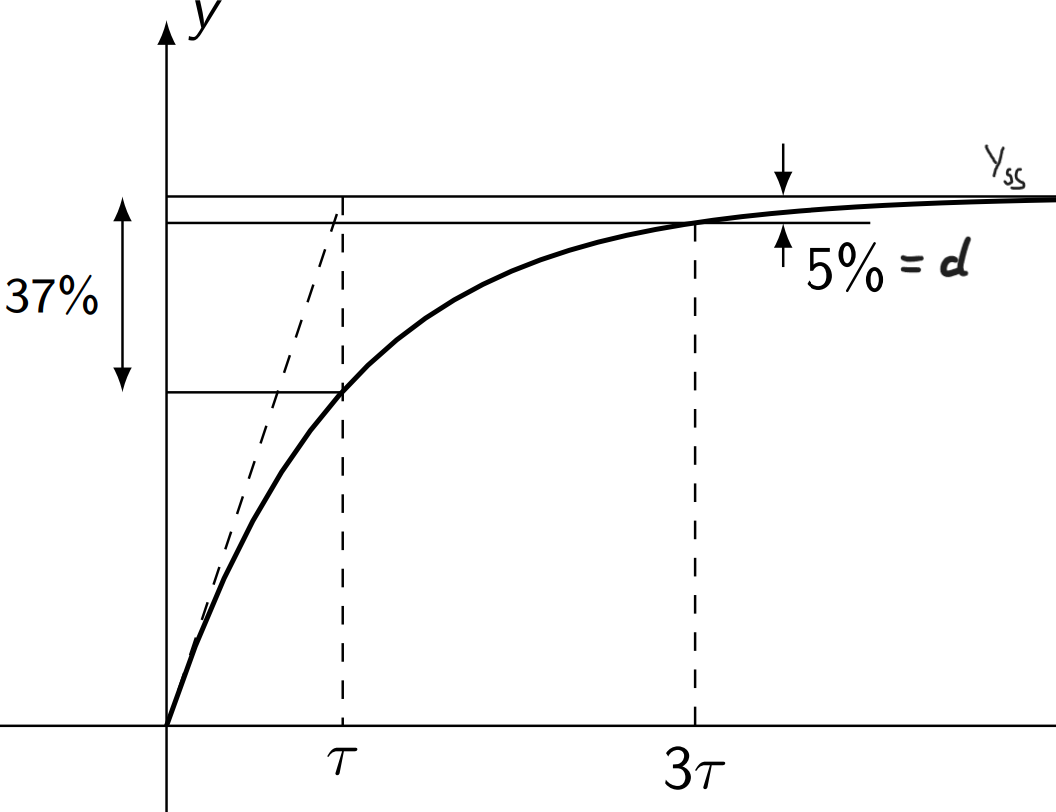
\includegraphics[width = \linewidth]{src/images/first_order_step_response.png}
    \subsubsection{Second Order System}
        \begin{align*}
            G(s) = \frac{\omega_n^2}{s^2 + 2 \zeta \omega_n s + \omega_n^2}\\
            \Leftrightarrow 
            \begin{cases*}
                \dot{x} = 
                    \left[\begin{array}{c c}
                        0 & 1\\
                        -\omega_n^2 & -2 \zeta \omega_n
                    \end{array}\right]
                    x + 
                    \left[\begin{array}{c}
                        0\\
                        \omega_n^2
                    \end{array}\right] u\\
                y = x
            \end{cases*}\\
            \Rightarrow y(t) = 1 - \frac{1}{cos(\varphi)}e^{\sigma t} cos(\omega t + \varphi)\\
            T_d = \tau \ln(100/d)\\
            \tau = \frac{1}{|\sigma|}\\
            \text{Time to peak: } T_p = \frac{\pi}{\tau}\\
            \text{Peak overshoot (ratio): } M_p = e^{\frac{\sigma \pi}{\omega}} \Rightarrow \zeta^2 = \frac{\ln(M_p)^2}{\pi^2 + \ln(M_p)^2}\\
            \text{Rise time: } T_{100 \%} = \frac{\frac{\pi}{2} - \varphi}{\omega} \approx \frac{\pi}{2 \omega_n}
        \end{align*}
        \titel{Nomenclature}
        \tikzset{
    pattern size/.store in=\mcSize, 
    pattern size = 5pt,
    pattern thickness/.store in=\mcThickness, 
    pattern thickness = 0.3pt,
    pattern radius/.store in=\mcRadius, 
    pattern radius = 1pt}
    \makeatletter
    \pgfutil@ifundefined{pgf@pattern@name@_9395wxxuh}{
    \pgfdeclarepatternformonly[\mcThickness,\mcSize]{_9395wxxuh}
    {\pgfqpoint{-\mcThickness}{-\mcThickness}}
    {\pgfpoint{\mcSize}{\mcSize}}
    {\pgfpoint{\mcSize}{\mcSize}}
    {
    \pgfsetcolor{\tikz@pattern@color}
    \pgfsetlinewidth{\mcThickness}
    \pgfpathmoveto{\pgfpointorigin}
    \pgfpathlineto{\pgfpoint{0}{\mcSize}}
    \pgfusepath{stroke}
}}
\makeatother
% Pattern Info
\tikzset{
    pattern size/.store in=\mcSize, 
    pattern size = 5pt,
    pattern thickness/.store in=\mcThickness, 
    pattern thickness = 0.3pt,
    pattern radius/.store in=\mcRadius, 
    pattern radius = 1pt}
    \makeatletter
    \pgfutil@ifundefined{pgf@pattern@name@_r1aowurqw}{
    \pgfdeclarepatternformonly[\mcThickness,\mcSize]{_r1aowurqw}
    {\pgfqpoint{-\mcThickness}{-\mcThickness}}
    {\pgfpoint{\mcSize}{\mcSize}}
    {\pgfpoint{\mcSize}{\mcSize}}
    {
    \pgfsetcolor{\tikz@pattern@color}
    \pgfsetlinewidth{\mcThickness}
    \pgfpathmoveto{\pgfpointorigin}
    \pgfpathlineto{\pgfpoint{0}{\mcSize}}
    \pgfusepath{stroke}
}}
\makeatother
\tikzset{every picture/.style={line width=0.75pt}} %set default line width to 0.75pt        

\begin{minipage}{0.64\linewidth}
    \def\imgx{175} %\insert linewidth
    \def\imgy{382/618 * \imgx} %golden ratio
    \begin{center} 
        \begin{tikzpicture}[x=0.75pt,y=0.75pt,yscale=-1,xscale=1]            
            %Axis
            %Re
            \draw[->] (0,\imgy*0.9) -- (\imgx,\imgy*0.9);
            \draw (\imgx, 0.9*\imgy) node [anchor = north] [font=\footnotesize] [align=left] {Re};
            %Im
            \draw[->] (\imgx*0.9,\imgy) -- (\imgx*0.9,0);
            \draw (0.9*\imgx, 0) node [anchor = west] [font=\footnotesize] [align=left] {Im};

    
            %Arrow
            \draw [->] (\imgx*0.9, \imgy*0.9) -- (\imgx*0.2, \imgy*0.2); %Arrow \omega_n
            \draw (0.2*\imgx, 0.2*\imgy) node [anchor = south east] [font=\footnotesize] [align=left] {$\omega_n$};

            %Dotted lines
            %\omega
            \draw[dotted] (\imgx*0.2, \imgy*0.2) -- (\imgx*0.9, \imgy*0.2);% \omega
            \draw (0.9*\imgx, 0.2*\imgy) node [anchor = west] [font=\footnotesize] [align=left] {$\omega$};
            %\sigma
            \draw[dotted] (\imgx*0.2, \imgy*0.32) -- (\imgx*0.2, \imgy*0.9);% \sigma
            \draw (0.2*\imgx, 0.9*\imgy) node [anchor = north] [font=\footnotesize] [align=left] {$\sigma$};

    
            %Angle
            \draw (\imgx*0.9,\imgy*0.9) -- (\imgx*0.9,\imgy*0.5) arc
                                    [
                                        start angle=-90,
                                        end angle=-148,
                                        x radius=\imgx*0.3,
                                        y radius=\imgy*0.3
                                    ];
            \draw (0.77*\imgx, 0.68*\imgy) node [anchor = west] [font=\footnotesize] [align=left] {$|\varphi|$};
        \end{tikzpicture}
    \end{center}
\end{minipage}
\begin{minipage}{0.34\linewidth}
    \begin{align*}
        |\omega_n| = \sqrt{\sigma^2 + \omega^2}\\
        |\sigma| = \zeta \omega_n\\
        \varphi = \arctan{\frac{\sigma}{\omega}}\\
        \zeta = \sin(|\varphi|)
    \end{align*}
\end{minipage}
        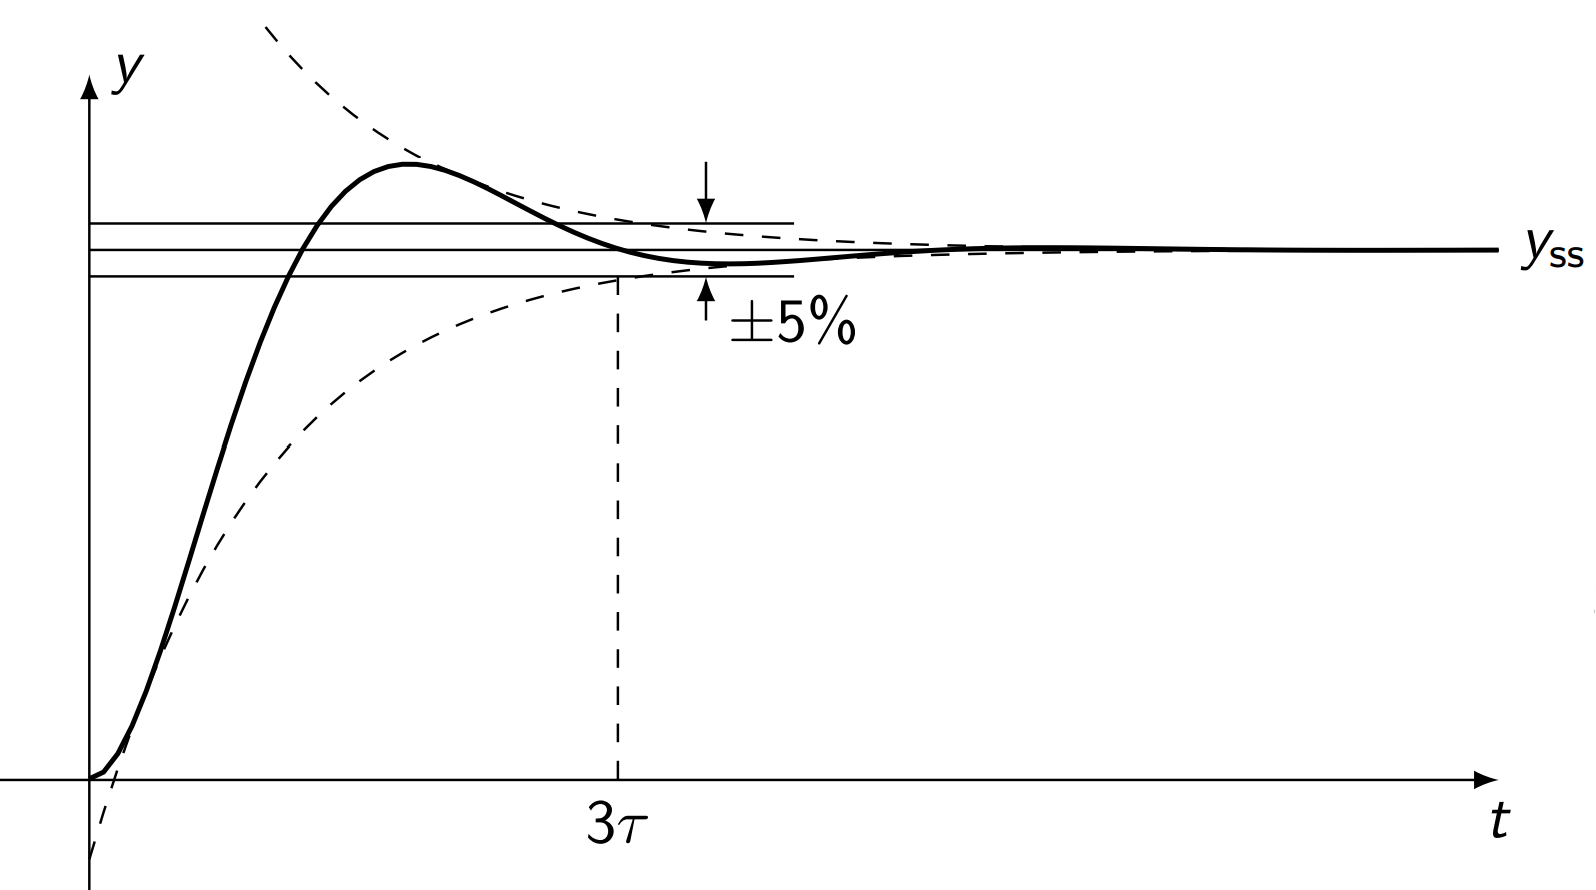
\includegraphics[width = \linewidth]{src/images/second_order_step_response.png}

	\subsection{Dominant poles approximation}
    Poles with the least negative part decay the slowest and are therefore considered \textbf{dominant}\\
    $G(s) = \frac{130}{(s+5) (s+1) (s+0.5)} \approx \frac{26}{(s+1) (s+0.5)} = G_{\text{dom}}, G_{\text{dom}}(0) \overset{\!}{=} G(0)$\\
    Pole-Zero cancellation with $p \approx z$ can be executed using the same method
	\subsection{Root Locus}
\begin{minipage}{0.49\linewidth}
    \begin{align*}
        k L(s) &= k\frac{N(s)}{D(s)}
    \end{align*}
\end{minipage}
\begin{minipage}{0.49\linewidth}
    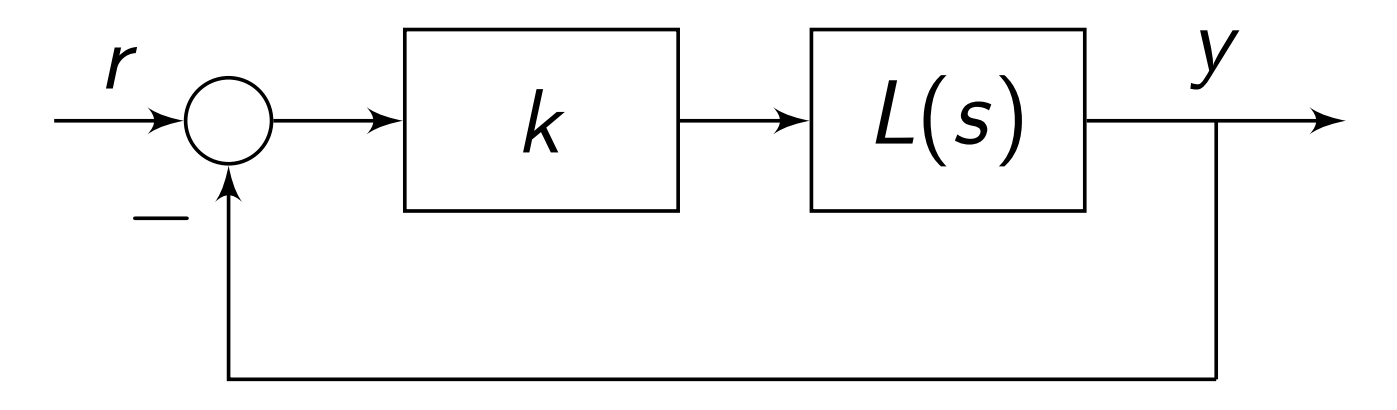
\includegraphics[width = \linewidth]{src/images/closed_loop.png}
\end{minipage}
\begin{align*}
    T(s) &= \frac{k L(s)}{1 + k L(s)} = \frac{k N(s)}{D(s) + k N(s)}
\end{align*}

\subsubsection{angle and magnitude rule}
\begin{align*}
    &\text{characteristic equation: } D(s) + kN(s) = 0\\
    &\Leftrightarrow \frac{N(s)}{D(s)} = L(s) = -\frac{1}{k}\\
    &\Rightarrow |L(s)| = \frac{1}{|k|} \quad \quad \quad
    \Rightarrow \angle(L(s)) = 
    \begin{cases}
        180 \text{° if } k > 0\\
        0 \text{° if } k < 0
    \end{cases}
\end{align*}

\subsubsection*{drawing the root locus}
\begin{itemize}
    \item closed-loop poles symmetric wrt real axis
    \item \# closed-loop poles = \# open-loop poles
    \item $k \rightarrow 0$: closed-loop poles approach open-loop poles
    \item $k \rightarrow \infty$: closed-loop poles approach open-loop zeros
    \item $n$ lines where $n =$ degree of D(s) or N(s), whichever greater
    \item no line crosses itself
    \item lines on the left of every odd numbered zero / pole (counting from right) (    o-----x    , x is 1st, o is 2nd, inverted for $k_{\text{bode}} < 0$)
    \item lines break out / in at 90°
    \item lines go to infinity along asymptotes with $\phi$ and centroid $c$ 
    \item $k < 0$: reverse rule 7 and add 180° to asymptotes
\end{itemize}
\begin{align}
    n = \# \text{poles}, m = \# \text{zeros}, q = 0, 1, 2 \dots (n-m-1)\\
    \phi = \frac{2q + 1}{n-m} \cdot 180^{\circ}, c = \frac{\sum\text{finite poles}}{\sum\text{finite zeros}}
\end{align}
	\subsection{Bode Plots}
    \subsubsection{Decibel scale}
        $z_{\text{dB}} = 20 * \log_{10}(z_{\text{decimal}}), 1 = 0dB, 10 = 20 dB, 100 = 40 dB$
    
    \subsubsection{Drawing the Bode plot}
        \begin{tabu}{| X | X | X |}
            \hline
            pole / zero type & change in magnitude & phase shift\\
            \hline \hline
            BIBO stable pole or integrator 1/s & -20dB/dec & $-90^{\circ}$\\
            \hline
            BIBO unstable pole & -20dB/dec & $+90^{\circ}$\\
            \hline
            minimum phase zero or differentiator s & +20dB/dec & $+90^{\circ}$\\
            \hline
            non-minimum phase zero & +20dB/dec & $-90^{\circ}$\\
            \hline
        \end{tabu}
        \begin{itemize}
            \item Slope of magnitude changes at pole / zero
            \item angle changes within a decade before and afer the pole/zero
            \item For $G(s)$ with incoming slope: calculate $|G(j \omega)|$ for $\omega = 1$
        \end{itemize}

    \subsubsection{Adding Bode Plots}
        Bode plot of $T(s) = k_1 \cdot T_1(s) + k_2 \cdot T_2(s)$ with given bode plots of $T_1(s)$ and $T_2(s)$:
        Bode plot of $T(s)$ is the addition of the Bode plots of $T_1(s)$ and $T_2(s)$ with respect to $k_1, k_2$

    \subsubsection{Inverted Transfer Function}
        Bode plot $T^{-1}(s)$ is the Bode plot $T(s)$ reflected about horizontal axis

    \subsubsection{Stability in Bode Plots}
        \begin{minipage}{0.64 \linewidth}
            \titel{crossover frequency, phase and gain margin}
                Bode plot of open loop system $\rightarrow$ closed loop Gain and Phase margin
                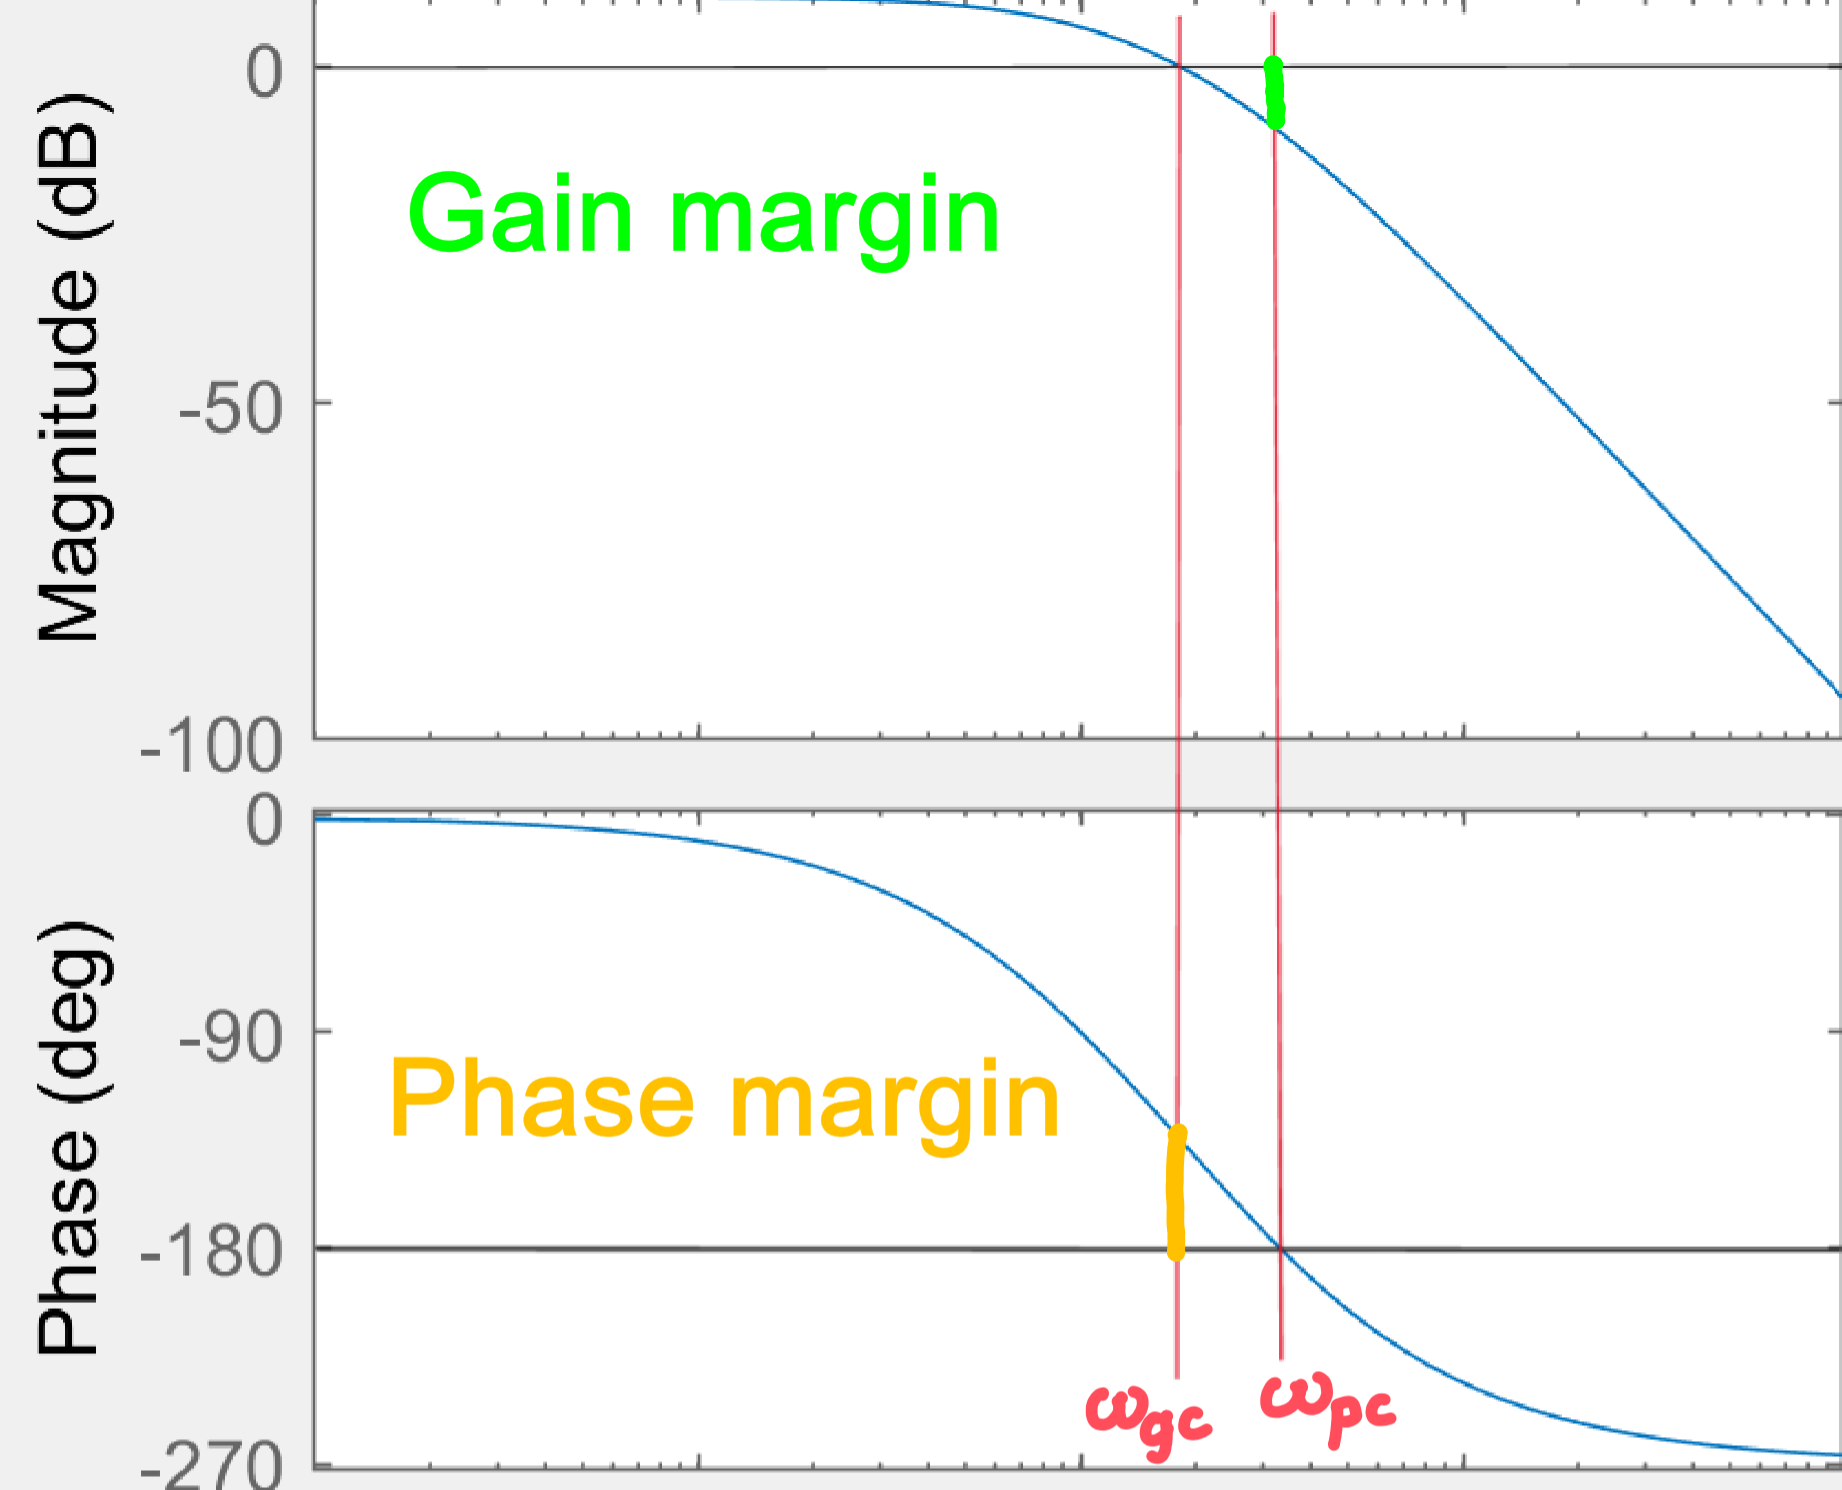
\includegraphics[width = \linewidth]{src/images/gain_phase_margin.png}
        \end{minipage}
        \begin{minipage}{0.34 \linewidth}
            \titel{stability criterion}
            For \textbf{\textit{stable}} open loop systems, the Nyquist criterion shows that the following must hold:
            \begin{align*}
                |G(j \omega_{pc})| < 0 dB\\
                \angle(G(j \omega_{pc})) > -180^{\circ}
            \end{align*}
            Crossover frequency:
            \begin{align*}
                \omega_{c} \Leftrightarrow |L(\omega_c)| = 0dB
            \end{align*}
        \end{minipage}

    

    \subsubsection{Bandwidth}
        maximum $\omega$ for which $|T(s)| > \frac{1}{\sqrt{2}}$
        Bandwidth is highest frequency a system can handle. Closed loop bandwidth $\approx$ open loop crossover frequency
        
%	\subsection{Polar plot}
    resulting from Bode plot: Draw every magnitude and corresponding angle in a polar coordinate system
	\subsection{Nyquist Plot}
    \begin{minipage}{0.49\linewidth}
        reflect the polar plot about the horizontal axis ($\omega$ is extended to negative values)

    \subsubsection{Nyquist condition}
        $Z = N + P$, Z = closed loop unstable poles, N = number of clockwise encirclements of the point $-\frac{1}{k}$, P = number of open loop unstable poles, no unstable pole / zero cancellation
    \end{minipage}
    \begin{minipage}{0.49\linewidth}
        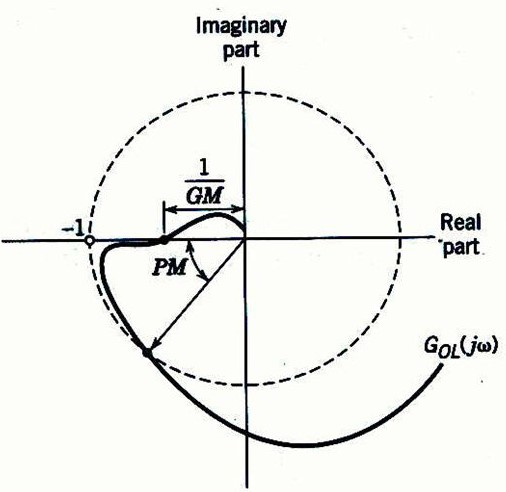
\includegraphics[width = \linewidth]{src/images/nyquist_gm_pm.jpg}
    \end{minipage}
    
    
	\subsection{Time Delay}
    $y(t) = e^{s(t-T)} = e^{-sT} u(t) \rightarrow$ Time delay is given by $e^{-sT} \overset{\text{Padé}}{\approx} \frac{\frac{2}{T} - s}{\frac{2}{T} + s}$\\
    Magnitude plot stays the same, angle goes to $-\infty$ for increasing $\omega$
	\subsection{retlative Degree $r$}
\vspace*{-1em}
    \begin{align*}
        r = \# p - \# z \Rightarrow \quad \text{Slope in Bode for }\lim\limits_{\omega \rightarrow \infty} \rightarrow \text{relative degree}\\
        r \geq 0: \text{realizable system}, r = 0 \rightarrow \text{ jump in step response at } t_0
    \end{align*}

\section{System Manipulation}
	\subsection{PID Controller}
    \subsubsection{P-Controller}
        \titel{Gain}
            \begin{align*}
                y(t) = u(t)
            \end{align*}
        \begin{itemize}
            \item proportional to error
            \item higher proportional gain moves crossover frequency up
            \item $k_P$ increases:
            \begin{itemize}
                \item closed-loop system of 2nd and higher order become more oscillatory
                \item closed-loop system remains stable
                \item $e_{ss}$ decreases
                \item faster response
                \item increased sensitivity to noise
            \end{itemize}
        \end{itemize}

    \subsubsection{I-Controller (integral)}
        \titel{Integrator}
            \begin{align*}
                y(t) = \int u(t) dt = \int e^{st} dt = \frac{1}{s} \cdot e^{st} = \frac{1}{s} \cdot u(t)
            \end{align*}
            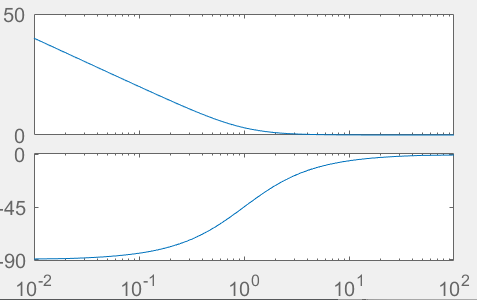
\includegraphics[width = \linewidth]{src/images/PI-controller.png}
        \begin{itemize}
            \item proportional to accumulated error
            \item new zero introduced
            \item number of asymptotes is reduced
            \item steady state error to step input\textbf{exactly zero}
            \item $k_I$ increases:
            \begin{itemize}
                \item more oscillatory response
                \item noise sensitivity does not change
            \end{itemize}
        \end{itemize}

    \subsubsection{D-Controller (derivative)}
        \titel{Differentiator}
            \begin{align*}
                y(t) = \frac{d u(t)}{dt} = \frac{d}{dt} e^{st} = s \cdot e^{st} = s \cdot u(t)
            \end{align*}
            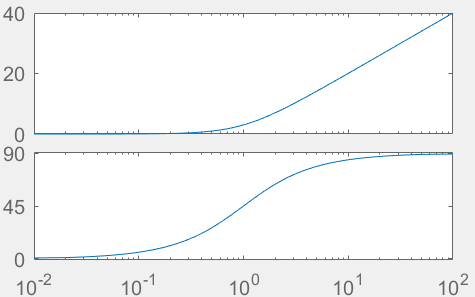
\includegraphics[width = \linewidth]{src/images/PD-controller.png}
        \begin{itemize}
            \item proportional to rate of change of error (reduced overshoot)
            \item pole introduced at $p=0$
            \item zero introduced at $z = -\frac{k_i}{k_p}$
            \item number of asymptotes unchanged
            \item $k_P$ increases:
            \begin{itemize}
                \item $e_{ss}$ unaffected
                \item less oscillatory, but potentially slower
                \item increased sensitivity to noise
            \end{itemize}
        \end{itemize}

    \subsubsection{Building the controller}
        \begin{minipage}{0.49\linewidth}
            \begin{align*}
                C(s) &= k_P + \frac{k_I}{s} + k_D \cdot s\\
                &= \frac{k_P \cdot s + k_I + k_D \cdot s^2}{s}\\
                &= k_P(1 + \frac{1}{T_I \cdot s} + T_D \cdot s)
            \end{align*}
        \end{minipage}
        \begin{minipage}{0.49\linewidth}
            \begin{scriptsize}
                \begin{align*}
                    k_P &= \text{Proportional gain}\\
                    k_I &= \text{Integral gain}\\
                    k_D &= \text{Derivative gain}\\
                    T_I &= \text{Integral time constant gain}\\
                    T_D &= \text{Derivative time constant}
                \end{align*}
            \end{scriptsize}
        \end{minipage}
        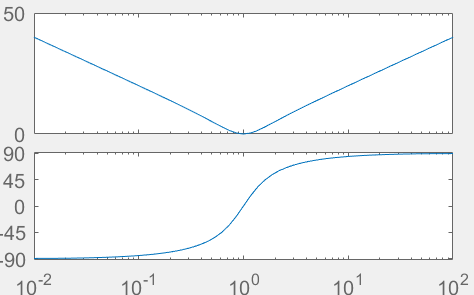
\includegraphics[width = \linewidth]{src/images/PID-controller.png}
        %Von ZF: P-controller, I-controller, D-controller
	\subsection{Lead- and Lag compensators}
    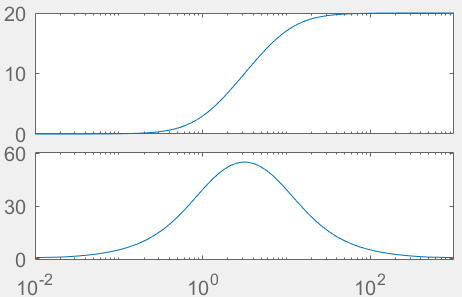
\includegraphics[width = \linewidth]{src/images/lead-controller.png}
    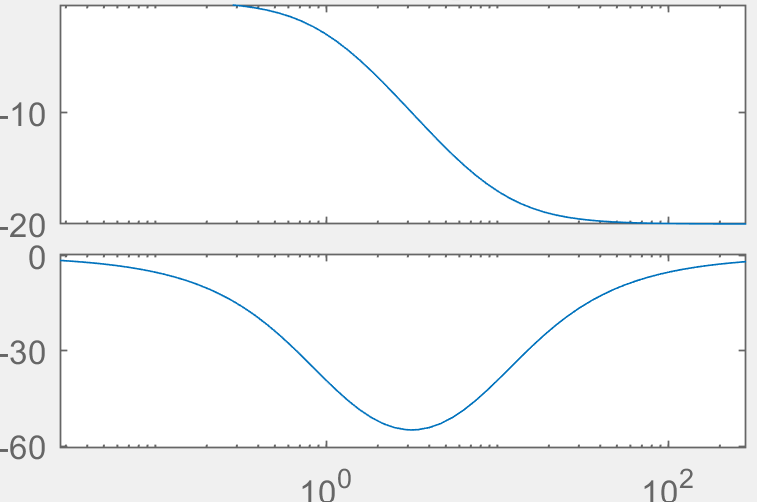
\includegraphics[width = \linewidth]{src/images/lag-controller.png}
	\subsection*{Non-minimum-phase / unstable system loop shaping}
\begin{align*}
    \text{For a plant: } P(s) = \frac{s - z}{s - p}, z > 0, p > 0\\
    P(s) = P_{\text{mp}}(s) \cdot D(s)\\
    P_{\text{mp}}(s) = \frac{s + z}{s + p}\\
    D(s) = \frac{z - s}{s + z} \cdot \frac{s + p}{s - p}\\
    \text{Non-minimum-phase: } \angle D(j \omega) = -2 \arctan(\frac{\omega}{z})\\
    \text{unstable pole: } \angle D(j \omega) = -2 \arctan(\frac{p}{\omega})
\end{align*}
$D(s)$ only changes phase of system, therefore design system for $P_{\text{mp}}(s)$ and adapt phase
	
\section{System Synthesis}
	\begin{itemize}
    \item larger gains / integrators reduce steady state error
    \item Open-loop-zeros attract, open-loop-poles repel closed-loop-poles
    \item place poles / zeros so that root locus goes through good region
\end{itemize}

draw requirements in graph for magnitude and phase\\
Build a controller using Gain k, integrator 1/s, Lead and lag compensator

\section{Nonlinear Systems}
	\subsection*{Jacobian Linearization of nonlinear Systems}
    \begin{align*}
        \frac{d}{dx} = f(x, u), \quad \quad y = h(x, u)\\
        \text{Equilibrium at state } \overline{x}: f(\overline{x}, \overline{u}) = 0\\
        \zeta = x - \overline{x}, \quad \quad \nu = u - \overline{u}\\
        \Rightarrow \frac{d}{dt} \zeta = \overline{f}(\zeta, \nu) \quad \quad y = \overline{h}(\zeta, \nu)
        \Rightarrow \overline{f}(0, 0) = 0, \quad \quad \overline{h}(0, 0) = \overline{y}\\
        \frac{d}{dt} \zeta \approx A \zeta + B \nu, \quad \quad y - \overline{y} \approx C \zeta + D \nu\\
        \begin{array}{c c}
            A = \frac{\partial \overline{f}(\zeta, \nu)}{\partial \zeta} \bigg|_{(0, 0)}       & B = \frac{\partial \overline{f}(\zeta, \nu)}{\partial \nu} \bigg|_{(0, 0)}\\
            C = \frac{\partial \overline{h}(\zeta, \nu)}{\partial \zeta} \bigg|_{(0, 0)}       & D = \frac{\partial \overline{h}(\zeta, \nu)}{\partial \nu} \bigg|_{(0, 0)}
        \end{array}
    \end{align*}
	\subsection{Cascaded Control}
    Two Outputs but only one input, E.g. Adaptive cruise control: speed, distance to mext car $\rightarrow$ throttle
	\subsection*{Integrator wind-up}
    When Input saturates (e.g. motor cannot create any more thrust), integral of error keeps increasing.\\
    Solution: Stop integrating, when input saturates:
    \begin{align*}
        k_I' = \begin{cases}
            k_I \text{if Input not saturated}\\
            0 \text{if Input saturated}
        \end{cases}
    \end{align*}
	\subsection{Robustness and uncertainty models}
    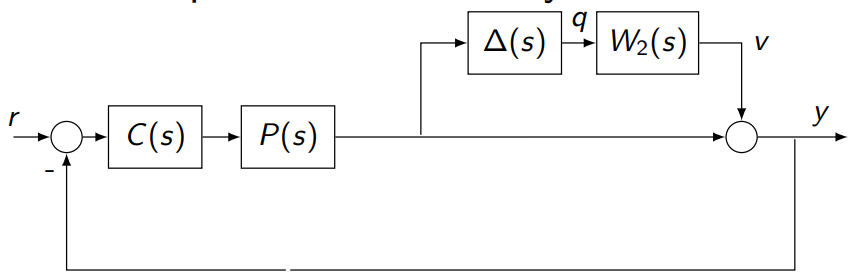
\includegraphics[width = \linewidth]{src/images/uncertainty_block_diagram.png}
    \begin{minipage}{0.58\linewidth}
        \begin{align*}
            &\tilde L(s) = (1 + W_2(s) \Delta(s)) P(s) C(s)\\
            &|\Delta| \leq 1 \quad \quad L(s) = P(s) C(s)\\
            &\Rightarrow |\tilde L(s) - L(s)|\\
            &= |W_2(s) \Delta(s) L(s)| \leq |W_2(s) L(s)|
        \end{align*}
        For $\tilde L$ not to encircle the -1 point, Nyquist plot of $L$ should never get closer than $|W_2(s) L(s)$ to -1 point:
        \begin{align*}
            |L(s) + 1| > |W_2(s) L(s)|
        \end{align*}
    \end{minipage}
    \begin{minipage}{0.40\linewidth}
        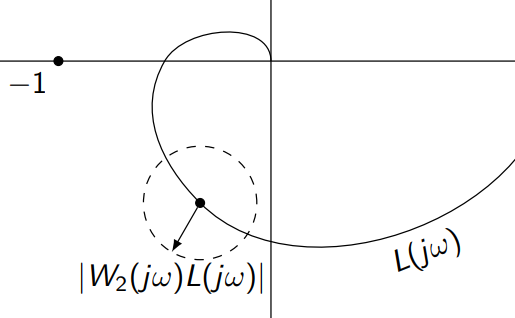
\includegraphics[width = \linewidth]{src/images/uncertainty_nyquist.png}
    \end{minipage}

\section{Appendix}
	\subsection{compute matrix exponential}
    \subsubsection{Taylor expansion}
        \begin{align*}
            e^{At} = I + At + \frac{1}{2}(At)^2 + ... + \frac{1}{n!}(At)^n + ...
        \end{align*}
    \subsubsection{Diagonalization}
        \begin{align*}
            A &= TDT^{-1}\\
            \Rightarrow exp(At) &= T e^{Dt} T^{-1}\\
            &= T \text{diag}(e^{\lambda_1 t}, e^{\lambda_2 t}, ..., e^{\lambda_n t}) T^{-1}\\
            T &= (EV_1, EV_2, ..., EV_n)
        \end{align*}
    \subsubsection{Jordan matrix}
        \begin{align*}
            exp\left(
                \left[
                    \begin{array}{c c c}
                        \lambda & 1 & 0\\
                        0 & \lambda & 1\\
                        0 & 0 & \lambda
                    \end{array}
                \right]
                t
            \right)
            =
            \left[
                \begin{array}{c c c}
                    1 & t & \frac{1}{2!} t^2\\
                    0 & 1 & t\\
                    0 & 0 & 1
                \end{array}
            \right]
            e^{\lambda t}
        \end{align*}
	\subsection{Euler Formula}
    \begin{align*}
        &e^{js} = cos(js) + j sin(js)\\
        &cos(s) = \frac{e^{js} + e^{-js}}{2} \quad \quad sin(s) = \frac{e^{js} - e^{-js}}{2j}
    \end{align*}
	\subsection{cover-up method for partial fraction expansion}
    \begin{align*}
        f(x) = \frac{(x-1)(x+5)}{x(x+1)\colorbox{green}{$(x+2)$}} = \frac{A}{x} + \frac{B}{x+1} + \frac{C}{\colorbox{green}{$(x+2)$}}\\
        \colorbox{green}{$(x+2)$} = 0 \rightarrow x = \colorbox{red}{-2} \rightarrow C = \frac{(\colorbox{red}{$(-2)$}-1)(\colorbox{red}{$(-2)$}+5)}{(\colorbox{red}{$(-2)$})(\colorbox{red}{$(-2)$}+1)}
    \end{align*}

	\subsection{Initial and final value theorem}
    \titel{Initial value theorem}
        \begin{align*}
            \lim\limits_{t \rightarrow 0} y(t) = \lim\limits_{s \rightarrow \infty} s Y(s)
        \end{align*}
    \titel{Final value theorem}
        presupposed that \textbf{system is stable}
        \begin{align*}
            \lim\limits_{t \rightarrow \infty} y(t) = \lim\limits_{s \rightarrow 0} s Y(s)
        \end{align*}

\end{document}

\begin{comment}
SIMPLE LAPLACE
	derivative of a laplace function
	laplace of step function
	laplace of x^n

	!!! Disturbance and Noise rejection !!!
\end{comment}